%iffalse
\let\negmedspace\undefined
\let\negthickspace\undefined
\documentclass[journal,12pt,onecolumn]{IEEEtran}
\usepackage{cite}
\usepackage{amsmath,amssymb,amsfonts,amsthm}
\usepackage{algorithmic}
\usepackage{graphicx}
\usepackage{textcomp}
\usepackage{xcolor}
\usepackage{txfonts}
\usepackage{listings}
\usepackage{enumitem}
\usepackage{mathtools}
\usepackage{gensymb}
\usepackage{comment}
\usepackage[breaklinks=true]{hyperref}
\usepackage{tkz-euclide} 
\usepackage{listings}
\usepackage{gvv}                                        
%\def\inputGnumericTable{}                                 
\usepackage[latin1]{inputenc}     
\usepackage{xparse}
\usepackage{color}                                            
\usepackage{array}                                            
\usepackage{longtable}                                       
\usepackage{calc}                                             
\usepackage{multirow}
\usepackage{multicol}
\usepackage{hhline}                                           
\usepackage{ifthen}                                           
\usepackage{lscape}
\usepackage{tabularx}
\usepackage{array}
\usepackage{float}
\newtheorem{theorem}{Theorem}[section]
\newtheorem{problem}{Problem}
\newtheorem{proposition}{Proposition}[section]
\newtheorem{lemma}{Lemma}[section]
\newtheorem{corollary}[theorem]{Corollary}
\newtheorem{example}{Example}[section]
\newtheorem{definition}[problem]{Definition}
\newcommand{\BEQA}{\begin{eqnarray}}
\newcommand{\EEQA}{\end{eqnarray}}
\usepackage{float}
%\newcommand{\define}{\stackrel{\triangle}{=}}
\theoremstyle{remark}
\usepackage{ circuitikz }
%\newtheorem{rem}{Remark}
% Marks the beginning of the document

\title{GATE-IN-2008}
\author{EE25BTECH11002 - Achat Parth Kalpesh }
\date{}

\begin{document}

\maketitle

\section*{Questions 1-20 (1 mark each)}
\begin{enumerate}
    \item Given y = $x^2$ + 2x + 10 , the value of $\frac{dy}{dx}\Big|_{x=1}$ is equal to \hfill{(GATE-IN 2008)}
    \begin{multicols}{4}
    \begin{enumerate} 
        \item 0
        \item 4 
        \item 12 
        \item 13
    \end{enumerate}
    \end{multicols}
    
    \item $\lim_{x \to 0} \frac{\sin x}{x}$ is \hfill{(GATE-IN 2008)}
    \begin{multicols}{4}
    \begin{enumerate} 
        \item indeterminate
        \item  0
        \item  1
        \item $\infty$
    \end{enumerate}
    \end{multicols}
    
    \item  The power supplied by the dc voltage source in the circuit shown below is \figref{fig:placeholder1} \hfill{(GATE-IN 2008)}
    
    \begin{figure}[H]
    \centering
    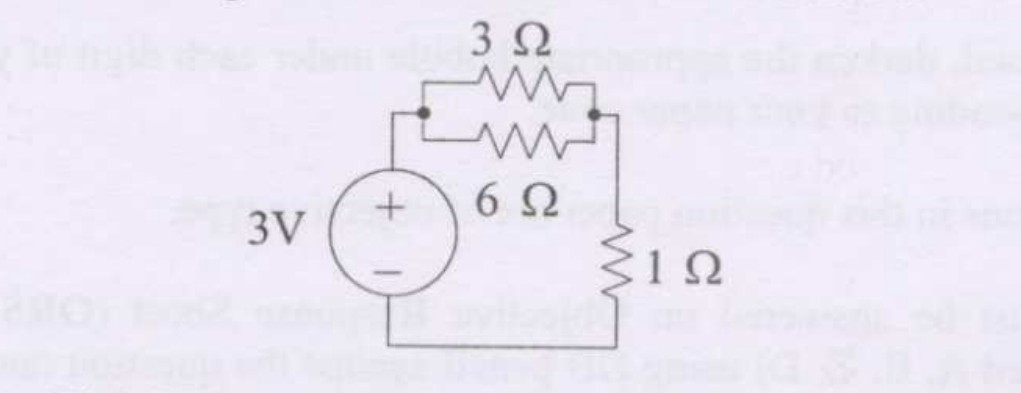
\includegraphics[width=0.5\columnwidth]{figs/i1.jpg}
    \caption{}
    \label{fig:placeholder1}
\end{figure}
\begin{multicols}{4}
        \begin{enumerate} 
        \item 0 W
        \item 1.0 W
        \item 2.5 W 
        \item 3.0 W
    \end{enumerate}
    \end{multicols}
    
    \item  The current I supplied by the dc voltage source in the circuit shown below is \figref{fig:placeholder2} \hfill{(GATE-IN 2008)}

 \begin{figure}[H]
    \centering
    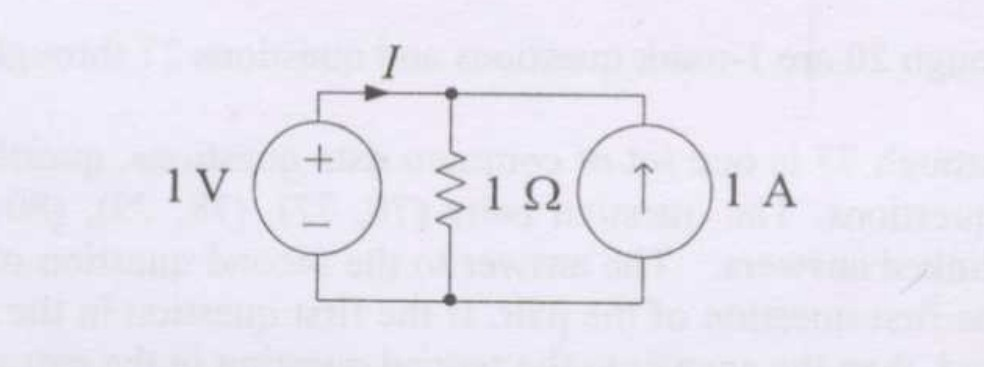
\includegraphics[width=0.5\columnwidth]{figs/i2.jpg}
    \caption{}
    \label{fig:placeholder2}
\end{figure}
\begin{multicols}{4}
    \begin{enumerate} 
        \item  0 A
        \item  0.5 A
        \item  1 A
        \item  2 A
    \end{enumerate}
    \end{multicols}
    \item For signal conditioning of a piezoelectric type transducer we require \hfill{(GATE-IN 2008)}
    \begin{multicols}{2}
    \begin{enumerate}
        \item a charge amplifier 
        \item  a differential amplifier
        \item  an instrumentation amplifier
        \item  a transconductance amplifier
    \end{enumerate}
    \end{multicols}
    
    \item A linear variable differential transformer \brak{LVDT} is \hfill{(GATE-IN 2008)}
    \begin{multicols}{2}
    \begin{enumerate} 
        \item a displacement transducer 
        \item an impedance matching transformer
        \item a differential temperature sensor
        \item an auto transformer
    \end{enumerate}
    \end{multicols}
    
    \item The temperature being sensed by a negative temperature coefficient \brak{NTC} type thermistor is linearly increasing. Its resistance will \hfill{(GATE-IN 2008)}
    \begin{multicols}{2}
    \begin{enumerate} 
        \item linearly increase with temperature
        \item exponentially increase with temperature 
        \item linearly decrease with temperature
        \item exponentially decrease with temperature
    \end{enumerate}
    \end{multicols}
    
    \item For a single stage BJT common base amplifier,\hfill{(GATE-IN 2008)}
    \begin{enumerate} 
        \item current gain as well as voltage gain can be greater than unity
        \item current gain can be greater than unity but voltage gain is always less than unity 
        \item voltage gain can be greater than unity but current gain is always less than unity 
        \item current gain as well as voltage gain is always less than unity
    \end{enumerate}
    
    \item In the circuit shown below \figref{fig:placeholder3}, the ideality factor n of the diode is unity and the voltage drop across it
is 0.7 V. The dynamic resistance of the diode at room temperature is approximately  voltage gain can be greater than unity but current gain is always less than unity\hfill{(GATE-IN 2008)}

 \begin{figure}[H]
    \centering
    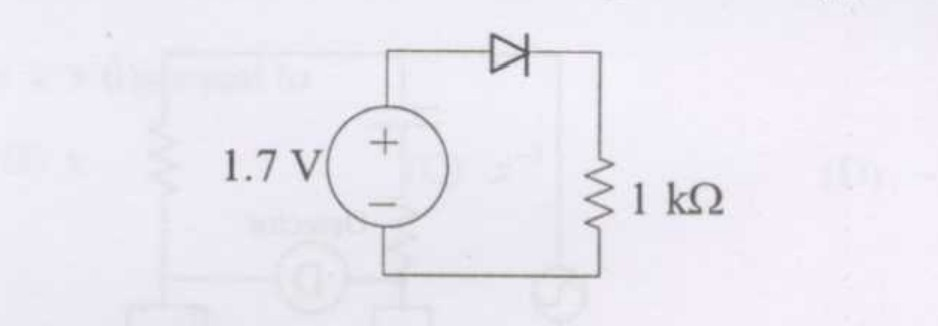
\includegraphics[width=0.5\columnwidth]{figs/i3.jpg}
    \caption{}
    \label{fig:placeholder3}
\end{figure}
\begin{multicols}{4}
    \begin{enumerate} 
        \item 15 $\ohm$
        \item 25 $\ohm$
        \item 50 $\ohm$
        \item 700 $\ohm$
    \end{enumerate}
    \end{multicols}
    
    \item An ideal op-amp has the characteristics of an ideal \hfill{(GATE-IN 2008)}
    \begin{multicols}{2}
    \begin{enumerate} 
        \item voltage controlled voltage source
        \item voltage controlled current source 
        \item current controlled voltage source 
        \item curremt controlled current source
    \end{enumerate}
    \end{multicols}
    
    \item The inverters in the ring oscillator circuit shown below \figref{fig:placeholder4} are identical. If the output waveform has a
frequency of 10 MHz, the propagation delay of each inverter is \hfill{(GATE-IN 2008)}
\begin{figure}[H]
    \centering
    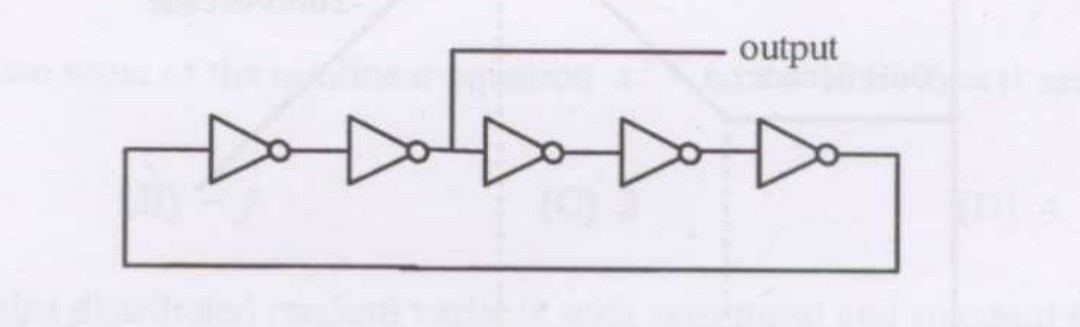
\includegraphics[width=0.5\columnwidth]{figs/i4.jpg}
    \caption{}
    \label{fig:placeholder4}
\end{figure}
\begin{multicols}{4}
    \begin{enumerate} 
        \item 5 ns
        \item 10 ns
        \item 20 ns
        \item 50 ns
    \end{enumerate}
    \end{multicols}
    
    \item A 2K$\times$8 bit RAM is interfaced to an 8-bit microprocessor. If the address of the first memory
location in the RAM is 0800H, the address of the last memory location will be \hfill{(GATE-IN 2008)}
\begin{multicols}{4}
    \begin{enumerate} 
        \item 1000H
        \item 0FFFH
        \item 4800H 
        \item 47FFH
    \end{enumerate}
    \end{multicols}
        
    \item  The fundamental period of the discrete-time signal
    $x$$\sbrak{n}$ = e$^{j(\frac{5\pi}{6})n}$ is  \hfill{(GATE-IN 2008)}
    \begin{multicols}{4}
    \begin{enumerate} 
        \item $\frac{6}{5\pi}$
        \item $\frac{12}{5}$
        \item 6
        \item 12
    \end{enumerate}
    \end{multicols}
    
    \item  Which one of the following discrete-time systems is time invariant? \hfill{(GATE-IN 2008)}
    \begin{multicols}{4}
    \begin{enumerate} 
        \item $y$$\sbrak{n}$ = $nx$$\sbrak{n}$
        \item $y$$\sbrak{n}$ = $x$$\sbrak{3n}$
        \item $y$$\sbrak{n}$ = $x$$\sbrak{-n}$
        \item $y$$\sbrak{n}$ = $x$$\sbrak{n-3}$
    \end{enumerate}
    \end{multicols}
    
    \item If a curent of $\sbrak{-6\sqrt{2}\sin\brak{100{\pi}t} +6\sqrt{2}\cos\brak{300{\pi}t + \frac{\pi}{4}} + 6\sqrt{2}}$   $A$ is passed through a true RMS ammeter , the meter reading will be \hfill{(GATE-IN 2008)} 
    \begin{multicols}{4}
    \begin{enumerate} 
        \item $6\sqrt{2}$ A
        \item $\sqrt{126}$ A
        \item 12 A
        \item $\sqrt{216}$ A
    \end{enumerate}
    \end{multicols}
    
    \item If the ac bridge circuit shown below \figref{fig:placeholder5} is balanced, the element Z can be a  \hfill{(GATE-IN 2008)}

\begin{figure}[H]
    \centering
    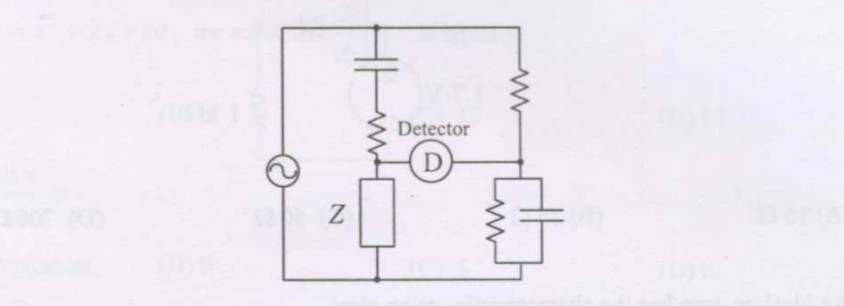
\includegraphics[width=0.5\columnwidth]{figs/i5.jpg}
    \caption{}
    \label{fig:placeholder5}
\end{figure}
    \begin{multicols}{2}
    \begin{enumerate} 
        \item pure capacitor
        \item pure inductor
        \item R-L series combination
        \item R-L parallel combination
    \end{enumerate}
    \end{multicols}
    
    \item The Bode asymptotic plot of a transfer function is given below\figref{fig:placeholder6}. In the frequency range shown, the
transfer function has \hfill{(GATE-IN 2008)}

\begin{figure}[H]
    \centering
    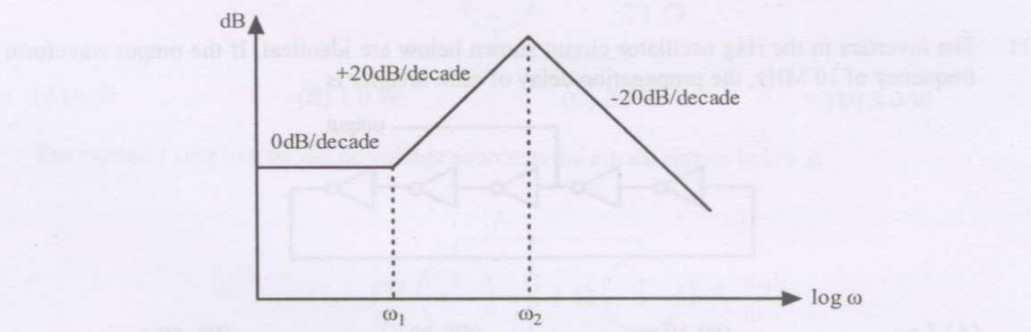
\includegraphics[width=0.5\columnwidth]{figs/i6.jpg}
    \caption{}
    \label{fig:placeholder6}
\end{figure}
\begin{multicols}{2}
    \begin{enumerate} 
        \item 3 poles and 1 zero 
        \item 1 pole and 2 zeros
        \item 2 poles and 1 zero 
        \item 2 poles and 2 zeros
    \end{enumerate}
    \end{multicols}
    
    \item For radioisotope imaging, an Anger camera is fitted with a parallel hole collimator. If the thickness
of the collimator is increased, the camera\hfill{(GATE-IN 2008)}
    \begin{enumerate} 
        \item  resolution and sensitivity will increase
        \item  resolution and sensitivity will decrease
        \item  resolution will increase and sensitivity will decrease
        \item  resolution will decrease and sensitivity will increase
    \end{enumerate}
    
    \item In the standard 12-lead ECG recording system, the minimum number of electrodes required to be
attached to a human subject for recording any one of the unipolar chest lead signals is \hfill{(GATE-IN 2008)}
\begin{multicols}{4}
    \begin{enumerate} 
        \item 1  
        \item 2
        \item 4
        \item 5
    \end{enumerate}
    \end{multicols}
    
    \item A laser light with a wavelength of 633 nm is passed through 1 cm length of tissue and 2 cm length
of glass. The refractive indices of tissue and glass are 1.33 and 1.5 respectively. The velocities of
laser light in the tissue and in the glass are in the ratio of \hfill{(GATE-IN 2008)}
\begin{multicols}{4}
    \begin{enumerate} 
        \item 1.33: 0.75
        \item 1.33: 3.0
        \item 1.33: 1.5
        \item 1.5: 1.33
    \end{enumerate}
    \end{multicols}

\section*{Questions 21-75 (2 marks each)}
    \item The expression $e^{-lnx}$ for $x > 0$ is equal to \hfill{(GATE-IN 2008)}
    \begin{multicols}{4}
    \begin{enumerate} 
        \item $-x$ 
        \item $x$
        \item $x^{-1}$ 
        \item $-x^{-1}$
    \end{enumerate}
    \end{multicols}
    
    \item Consider the differential equation $\frac{dy}{dx}=1 + y^2$. Which one of the following can be a particular solution of this differential equation? \hfill{(GATE-IN 2008)}
    \begin{multicols}{4}
    \begin{enumerate} 
        \item $y=tan\brak{x+3}$
        \item $y=tanx + 3$ 
        \item $x=tan\brak{y+3}$ 
        \item $x=tany + 3$
    \end{enumerate}
    \end{multicols}
    
    \item  Consider the function $y=x^2 -6x +9$.The maximum value of y obtained when x varies over the interval 2 to 5 is \hfill{(GATE-IN 2008)}
    \begin{multicols}{4}
    \begin{enumerate} 
        \item 1
        \item 3 
        \item 4 
        \item 9
    \end{enumerate}
    \end{multicols}
    
    \item It is known that two roots of the nonlinear equation $x^3 -6x^2 +11x -6 = 0$ are 1 and 3. The third root will be \hfill{(GATE-IN 2008)}
    \begin{multicols}{4}
    \begin{enumerate} 
        \item $j$ 
        \item $-j$
        \item 2
        \item 4
    \end{enumerate}
    \end{multicols}
    
    \item Consider a Gaussian distributed random variable with zero mean and standard deviation $\sigma$ . The
value of its cumulative distribution function at the origin will be \hfill{(GATE-IN 2008)}
\begin{multicols}{4}
    \begin{enumerate} 
        \item 0
        \item 0.5
        \item 1
        \item 10 $\sigma$
    \end{enumerate}
    \end{multicols}
    
    \item  A random variable is uniformly distributed over the interval 2 to 10. Its variance will be \hfill{(GATE-IN 2008)}
    \begin{multicols}{4}
    \begin{enumerate} 
        \item \(\frac{16}{3}\) 
        \item 6
        \item \(\frac{256}{9}\)
        \item 36
    \end{enumerate}
    \end{multicols}
    
    \item The Fourier transform of $x\brak{t}$ = $e^{-at}$$u\brak{-t}$, where $u\brak{t}$is the unit step function,\hfill{(GATE-IN 2008)}
    \begin{multicols}{2}
    \begin{enumerate} 
        \item exists for any real value of a
        \item does not exist for any real value of a
        \item exists if the real value of a is strictly negative
        \item exists if the real value of a is strictly positive
    \end{enumerate}
    \end{multicols}
    
    \item In the circuit shown below \figref{fig:placeholder7} the maximum power that can be transferred to the load ZL is \hfill{(GATE-IN 2008)}

        \begin{figure}[H]
    \centering
    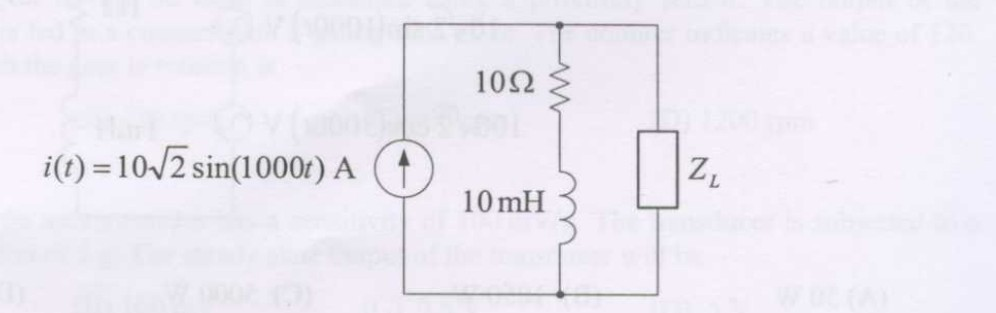
\includegraphics[width=0.5\columnwidth]{figs/i7.jpg}
    \caption{}
    \label{fig:placeholder7}
\end{figure}
\begin{multicols}{4}
    \begin{enumerate} 
        \item 250 W
        \item 500 W
        \item 1000 W
        \item 2000 W
    \end{enumerate}
    \end{multicols}
    
    \item A complex variable $Z=x + j0.1$ has its real part x varying in the range $-\infty$ to $\infty$ . Which of the following is the locus (shown in thick lines) of \(\frac{1}{Z}\) in the complex plane ? \hfill{(GATE-IN 2008)}
    \begin{multicols}{2}
    \begin{enumerate} 
        \item  
        
       \begin{figure}[H]
    \centering
    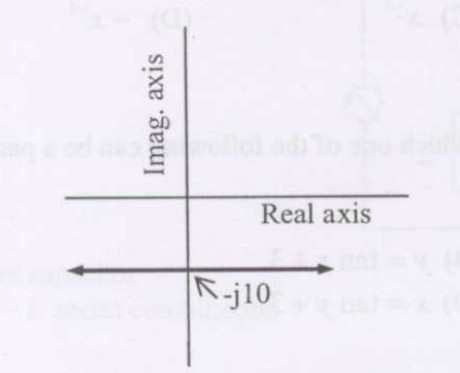
\includegraphics[width=0.5\columnwidth]{figs/i8.jpg}
    \caption{}
    \label{fig:placeholder8}
\end{figure}
        \item  

           \begin{figure}[H]
    \centering
    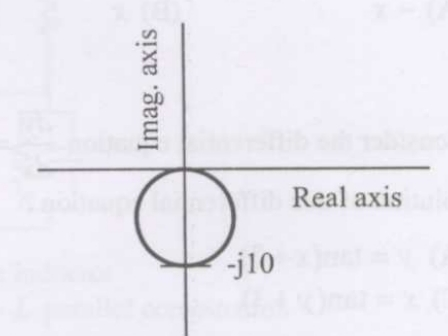
\includegraphics[width=0.5\columnwidth]{figs/i9.jpg}
    \caption{}
    \label{fig:placeholder9}
\end{figure}
        \item  

          \begin{figure}[H]
    \centering
    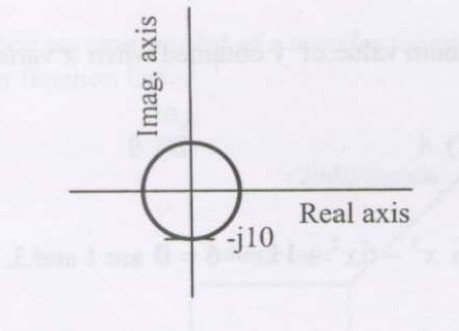
\includegraphics[width=0.5\columnwidth]{figs/i10.jpg}
    \caption{}
    \label{fig:placeholder10}
\end{figure}
        \item 

           \begin{figure}[H]
    \centering
    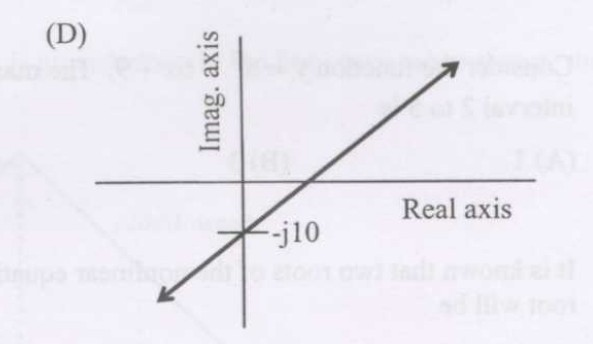
\includegraphics[width=0.5\columnwidth]{figs/i11.jpg}
    \caption{}
    \label{fig:placeholder11}
\end{figure}
    \end{enumerate}
    \end{multicols}
    
    \item For the circuit shown below\figref{fig:placeholder12} the input resistance $R_{11} = \frac{V_1}{I_1}\Big|_{I_2=0}$is \hfill{(GATE-IN 2008)}
  \begin{figure}[H]
    \centering
    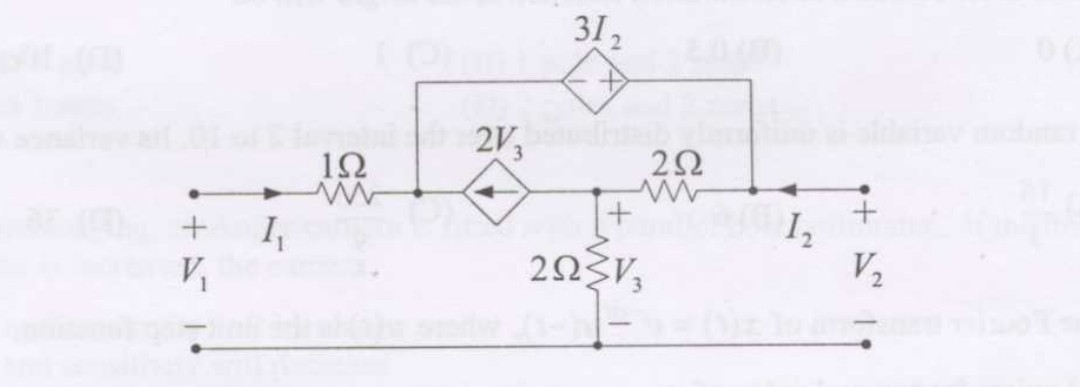
\includegraphics[width=0.5\columnwidth]{figs/i12.jpg}
    \caption{}
    \label{fig:placeholder12}
\end{figure}
\begin{multicols}{4}
    \begin{enumerate} 
        \item -3 $\ohm$
        \item  2 $\ohm$
        \item  3 $\ohm$
        \item 13 $\ohm$
    \end{enumerate}
    \end{multicols}
    
    \item In the circuit shown below \figref{fig:placeholder13} the average power consumed by the 1$\ohm$ resistor is \hfill{(GATE-IN 2008)}

  \begin{figure}[H]
    \centering
    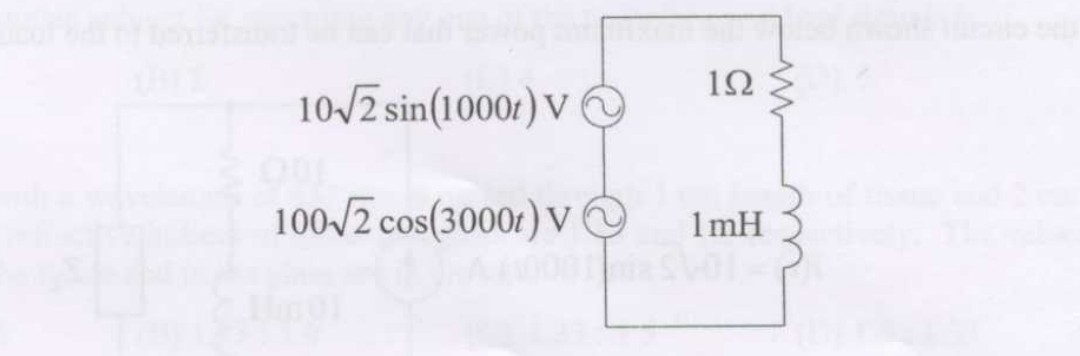
\includegraphics[width=0.5\columnwidth]{figs/i13.jpg}
    \caption{}
    \label{fig:placeholder13}
\end{figure}

\begin{multicols}{4}
    \begin{enumerate} 
        \item 50 W
        \item 1050 W
        \item 5000 W
        \item 10100 W
    \end{enumerate}
    \end{multicols}
    
    \item Which one of the following equations is valid for the circuit shown below? \figref{fig:placeholder14} \hfill{(GATE-IN 2008)}

       \begin{figure}[H]
    \centering
    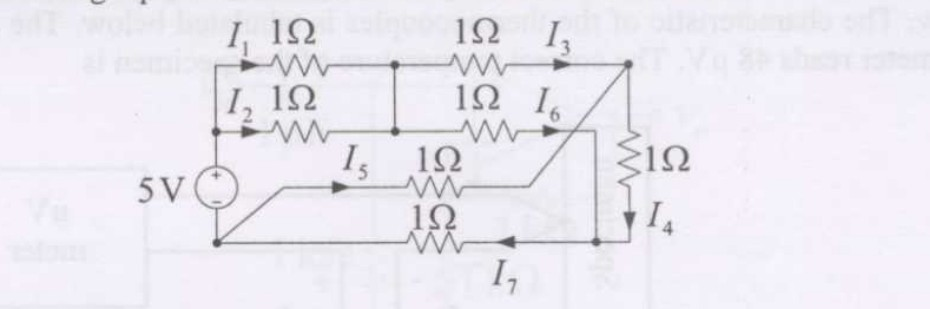
\includegraphics[width=0.5\columnwidth]{figs/i14.jpg}
    \caption{}
    \label{fig:placeholder14}
\end{figure}
\begin{multicols}{2}
    \begin{enumerate} 
        \item $I_3+ I_5- I_6+ I_7 = 0 $
        \item  $I_3- I_5+ I_6+ I_7 = 0 $
        \item $I_3+ I_5+ I_6+ I_7 = 0 $ 
        \item $I_3+ I_5+ I_6- I_7 = 0 $
    \end{enumerate}
    \end{multicols}
    
    \item  For the circuit shown below \figref{fig:placeholder15} the steady-state current I is \hfill{(GATE-IN 2008)}

   \begin{figure}[H]
    \centering
    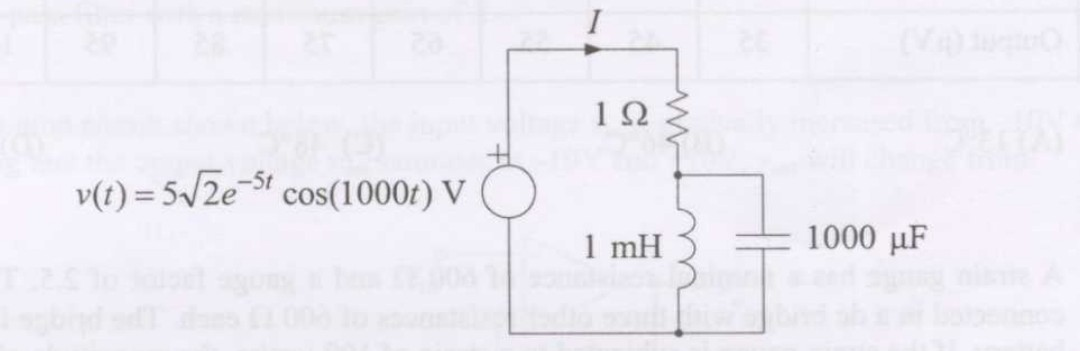
\includegraphics[width=0.5\columnwidth]{figs/i15.jpg}
    \caption{}
    \label{fig:placeholder15}
\end{figure}
\begin{multicols}{4}
    \begin{enumerate} 
        \item 0 A 
        \item $5\sqrt{2} \cos\brak{1000t} A$
        \item $5\sqrt{2} \cos\brak{1000t - \frac{\pi}{4}} A$
        \item $5\sqrt{2} A$
    \end{enumerate}
    \end{multicols}
    
    \item For the circuit shown below \figref{fig:placeholder16} the voltage across the capacitor is \hfill{(GATE-IN 2008)}

\begin{figure}[H]
    \centering
    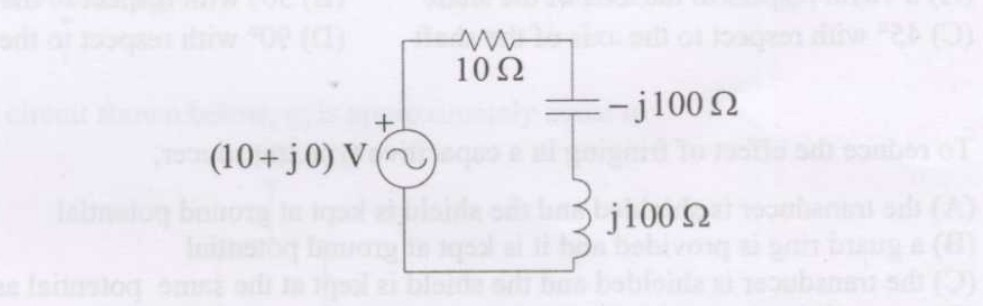
\includegraphics[width=0.5\columnwidth]{figs/i16.jpg}
    \caption{}
    \label{fig:placeholder16}
\end{figure}
\begin{multicols}{4}
    \begin{enumerate} 
        \item \brak{10+j0} V
        \item \brak{100+ j0} V 
        \item \brak{0+j100} V 
        \item \brak{0-j100} V
    \end{enumerate}
    \end{multicols}
    
    \item The speed of a gear having 60 teeth is measured using a proximity sensor. The output of the
proximity sensor is fed to a counter with a gating time of 1s. The counter indicates a value of 120.
The speed at which the gear is rotating is \hfill{(GATE-IN 2008)}
\begin{multicols}{4}
    \begin{enumerate} 
        \item 60 rpm 
        \item 120 rpm
        \item 600 rpm
        \item 1200 rpm 
    \end{enumerate}
    \end{multicols}
    
    \item A piezoelectric type accelerometer has a sensitivity of 100 mV/g. The transducer is subjected to a
constant acceleration of 5 g. The steady state output of the transducer will be \hfill{(GATE-IN 2008)}
\begin{multicols}{4}
    \begin{enumerate} 
        \item 0 V 
        \item 100 mV
        \item 0.5 V
        \item 5 V
    \end{enumerate}
    \end{multicols}
    
    \item A pair of identical thermocouples is employed for measuring the temperature of a specimen as shown below. \figref{fig:placeholder17} The characteristic of the thermocouples is tabulated below. The reference junction is at $2\degree$C. The meter reads 48 $\mu$V. The correct temperature of the specimen is \hfill{(GATE-IN 2008)}
    
\begin{figure}[H]
    \centering
    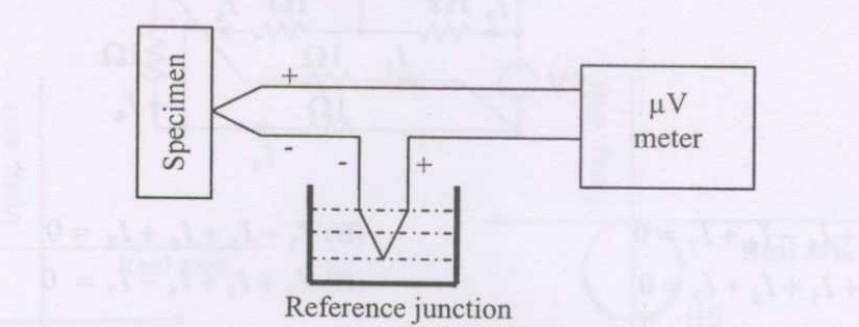
\includegraphics[width=0.5\columnwidth]{figs/i17.jpg}
    \caption{}
    \label{fig:placeholder17}
\end{figure}





\begin{table}[h]
\centering
\begin{tabular}{|l|c|c|c|c|c|c|c|c|c|c|}
\hline
Temperature $\brak{\degree C}$ & 0 & 10 & 20 & 30 & 40 & 50 & 60 & 70 & 80 & 90 \\
\hline
Output $\brak{\mu V}$ & 35 & 45 & 55 & 65 & 75 & 85 & 95 & 105 & 115 & 125 \\
\hline
\end{tabular}
\caption{}
\label{Table}
\end{table}








\begin{multicols}{4}
    \begin{enumerate} 
        \item  $13\degree$C
        \item  $46\degree$C
        \item  $48\degree$C
        \item  $50\degree$C
    \end{enumerate}
    \end{multicols}
    
    \item A strain gauge has a nominal resistance of 600$\ohm$ and a gauge factor of 2.5. The strain gauge is
connected in a dc bridge with three other resistances of 600$\ohm$ each. The bridge is excited by a 4 V
battery. If the strain gauge is subjected to a strain of 100 $\mu$m/m, the magnitude of the bridge output will be \hfill{(GATE-IN 2008)}
\begin{multicols}{4}
    \begin{enumerate} 
        \item  $0 V$
        \item  250 $\mu$V
        \item  500 $\mu$V
        \item  750 $\mu$V
    \end{enumerate}
    \end{multicols}
    
    \item The torque in a rotating shaft is measured using strain gauges. The strain gauges must be positioned
on the shaft such that the axes of the strain gauges are at \hfill{(GATE-IN 2008)}
\begin{multicols}{2}
    \begin{enumerate} 
        \item  $0\degree$ with respect to the axis of the shaft 
        \item  $30\degree$ with respect to the axis of the shaft
        \item  $45\degree$ with respect to the axis of the shaft
        \item  $90\degree$ with respect to the axis of the shaft
    \end{enumerate}
    \end{multicols}
    
    \item To reduce the effect of fringing in a capacitive type transducer, \hfill{(GATE-IN 2008)}
    \begin{enumerate} 
        \item  the transducer is shielded and the shield is kept at ground potential  
        \item  a guard ring is provided and it is kept at ground potential  
        \item   the transducer is shielded and the shield is kept at the same potential as the moving plate
        \item a guard ring is provided and it is kept at the same potential as the moving plate
    \end{enumerate}

    \item A differential amplifier shown below \figref{fig:placeholder18} has a differential mode gain of 100 and a CMRR of 40 dB. If $V_1$= 0.55V  and $V_2$ = 0.45 V, the output $V_0$ is \hfill{(GATE-IN 2008)}

 \begin{figure}[H]
    \centering
    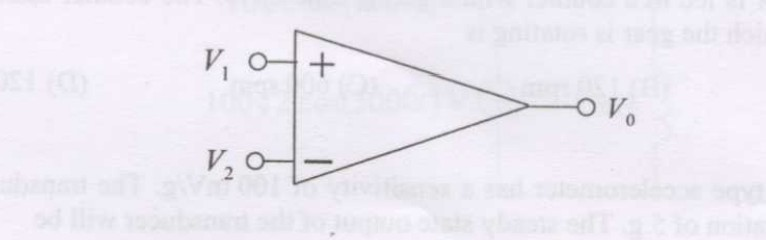
\includegraphics[width=0.5\columnwidth]{figs/i18.jpg}
    \caption{}
    \label{fig:placeholder18}
\end{figure}

\begin{multicols}{4}     
    \begin{enumerate} 
        \item 10 V 
        \item 10.5 V
        \item 11 V
        \item 15 V
    \end{enumerate}
    \end{multicols}
    

    \item  The op-amp circuit shown below \figref{fig:placeholder19} is that of a \hfill{(GATE-IN 2008)}
    \begin{figure}[H]
    \centering
    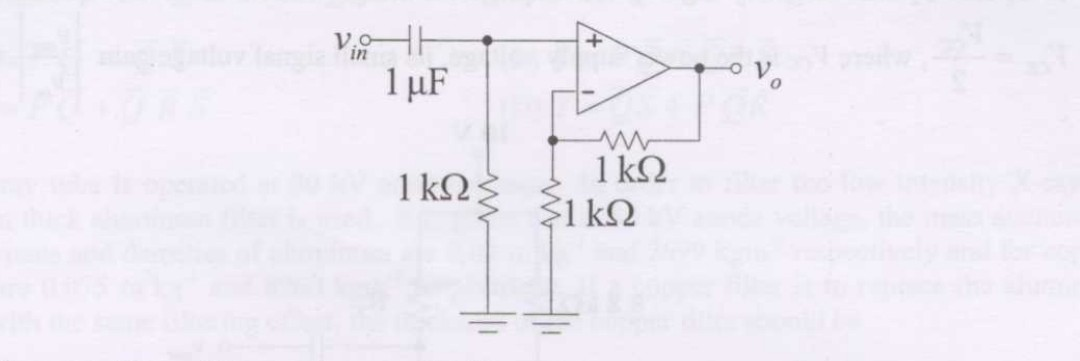
\includegraphics[width=0.5\columnwidth]{figs/i19.jpg}
    \caption{}
    \label{fig:placeholder19}
\end{figure}
\begin{multicols}{2}
    \begin{enumerate} 
        \item low-pass filter with a maximum gain of 1 
        \item low-pass filter with a maximum gain of 2
        \item high-pass filter with a maximum gain of 1 
        \item high-pass filter with a maximum gain of 2
    \end{enumerate}
    \end{multicols}
    
    \item In the op-amp circuit shown below \figref{fig:placeholder20}, the input voltage $v_{in}$ is gradually increased from -10V to +10V.Assuming that the output voltage $v_{out}$ saturates at -10V and +10V, $V_{out}$ will change from \hfill{(GATE-IN 2008)}
    
    \begin{figure}[H]
    \centering
    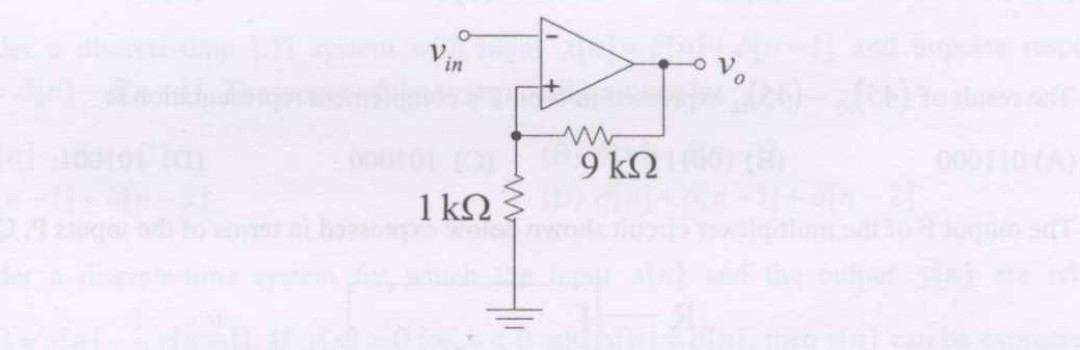
\includegraphics[width=0.5\columnwidth]{figs/i20.jpg}
    \caption{}
    \label{fig:placeholder20}
\end{figure}
\begin{multicols}{2}
    \begin{enumerate} 
        \item -10 V to +10 V when $v_{in}$ =-1 V
        \item -10 V to +10 V when $v_{in}$ = +1 V
        \item +10 V to -10 V when $v_{in}$ =-1 V
        \item +10 V to -10 V when $v_{in}$ = +1 V
    \end{enumerate}
    \end{multicols}
    
    \item  For the op-amp circuit shown below \figref{fig:placeholder21}, $v_0$ is approximately equal to \hfill{(GATE-IN 2008)}
    \begin{figure}[H]
    \centering
    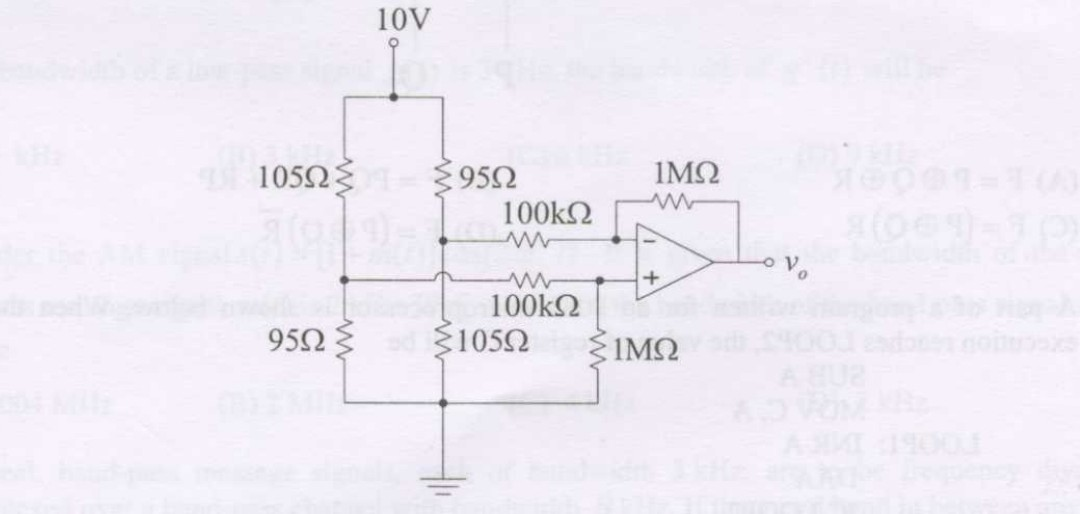
\includegraphics[width=0.5\columnwidth]{figs/i21.jpg}
    \caption{}
    \label{fig:placeholder21}
\end{figure}
\begin{multicols}{4}
    \begin{enumerate} 
        \item -10 V
        \item  -5 V
        \item  +5 V
        \item +10 V
    \end{enumerate}
    \end{multicols}
    
    \item  In the amplifier circuit shown below \figref{fig:placeholder22}, assume $V_{BE}$ = 0.7 V and the $\beta$ of the transistor and the values
of $C_1$ and $C_2$ are extremely high. If the amplifier is designed such that at the quiescent point its $V_{CE}$=$\frac{V_{CC}}{2}$ where $V_{CC}$  is the power supply voltage, its small signal voltage gain $\lvert \ \frac{V_{out}}{V_{in}}\  \rvert$ will be \hfill{(GATE-IN 2008)}
\begin{figure}[H]
    \centering
    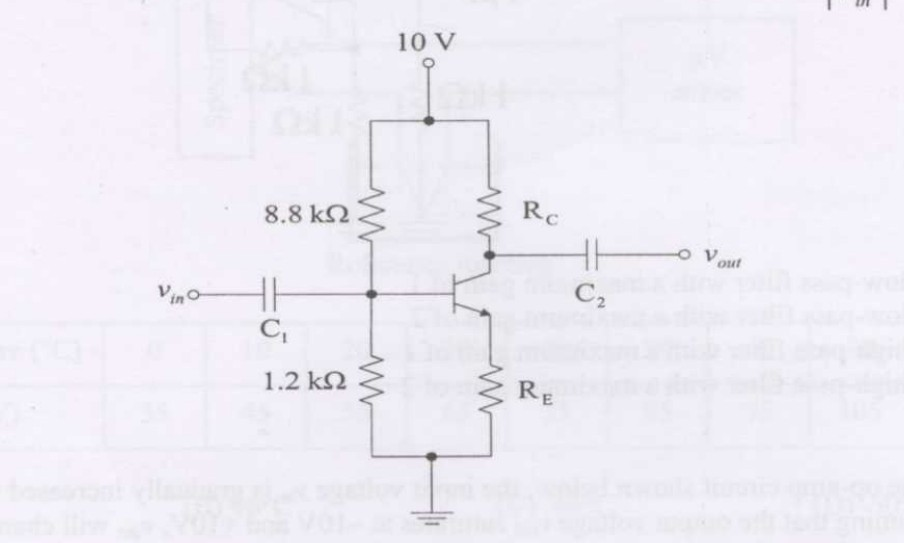
\includegraphics[width=0.5\columnwidth]{figs/i22.jpg}
    \caption{}
    \label{fig:placeholder22}
\end{figure}
\begin{multicols}{4}
    \begin{enumerate} 
        \item 3.75
        \item  4.5
        \item  9
        \item 19
    \end{enumerate}
    \end{multicols}
    
    \item The result of $(45)_{10}$ - $(45)_{16}$ expressed in 6-bit 2's complement representation is \hfill{(GATE-IN 2008)}
    \begin{multicols}{4}
    \begin{enumerate} 
        \item 011000
        \item 100111
        \item 101000
        \item 101001
    \end{enumerate}
    \end{multicols}
    
    \item  The output F of the multiplexer circuit shown below \figref{fig:placeholder23} expressed in terms of the inputs P, Q and R is \hfill{(GATE-IN 2008)}
    \begin{figure}[H]
    \centering
    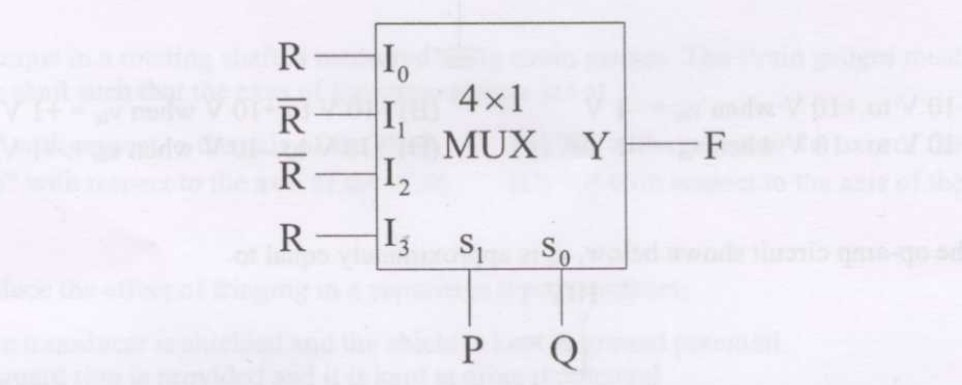
\includegraphics[width=0.5\columnwidth]{figs/i23.jpg}
    \caption{}
    \label{fig:placeholder23}
\end{figure}
\begin{multicols}{4}
    \begin{enumerate} 
        \item  F= P $\oplus$ Q $\oplus$ R
        \item  F = PQ + QR + RP
        \item  F= $\brak{P \oplus Q}R$
        \item  F =$\brak{P\oplus Q} \bar{R}$
    \end{enumerate}
    \end{multicols}
    
    \item A part of a program written for an 8085 microprocessor is shown below. When the program
execution reaches LOOP2, the value of register C will be

 SUB A\\ 
 MOV C, A  \\
 LOOP1: INR A\\  
    DAA  \\
    JC LOOP2\\  
    INR C  \\
    JNC LOOP1\\  
LOOP2: NOP\\
 \hfill{(GATE-IN 2008)}
 \begin{multicols}{4}
    \begin{enumerate} 
        \item 63 H
        \item 64 H
        \item 99 H
        \item 100 H
    \end{enumerate}
    \end{multicols}
    
    \item  The minimum sum of products form of the Boolean expression Y = $\bar{P}$$\bar{Q}$$\bar{R}$$\bar{S}$ + P$\bar{Q}$$\bar{R}$$\bar{S}$ + P$\bar{Q}$$\bar{R}$S + P$\bar{Q}$RS + P$\bar{Q}$R$\bar{S}$ + $\bar{P}$$\bar{Q}$R$\bar{S}$ \hfill{(GATE-IN 2008)}
    \begin{multicols}{2}
    \begin{enumerate} 
        \item  Y = P$\bar{Q}$ + $\bar{Q}$$\bar{S}$
        \item  Y = P$\bar{Q}$ + $\bar{Q}$R$\bar{S}$
        \item  Y = P$\bar{Q}$ + $\bar{Q}$$\bar{R}$$\bar{S}$
        \item  Y = $\bar{Q}$$\bar{S}$ + P$\bar{Q}$R
    \end{enumerate}
    \end{multicols}
    
    \item An X-ray tube is operated at 80 kV anode voltage. In order to filter the low intensity X-rays, a
2.5 mm thick aluminum filter is used. It is given that at 80 kV anode voltage, the mass attenuation
coefficients and densities of aluminum are $0.02$ $\text{m}^{2}\,\text{kg}^{-1}$ and 2699 $\text{kg}\,\text{m}^{-3}$ respectively and for copper
these are 0.075 $\text{m}^{2}\,\text{kg}^{-1}$ and 8960 $\text{kg}\,\text{m}^{-3}$ respectively. If a copper filter is to replace the aluminum
filter with the same filtering effect, the thickness of the copper filter should be \hfill{(GATE-IN 2008)}
\begin{multicols}{4}
    \begin{enumerate} 
        \item 0.2 mm
        \item 0.66 mm
        \item 1.5 mm
        \item 5 mm
    \end{enumerate}
    \end{multicols}
    
    
    
    \item A 5 MHz acoustic pulse travels from a transducer through a 2 cm thick fat tissue before it
encounters an interface with a liver tissue at normal incidence. The amplitude attenuation factors of
fat and liver are 0.075 $\text{Np}\,\text{cm}^{-1}/MHz$ and 0.1 $\text{Np}\,\text{cm}^{-1}/MHz$ respectively. The amplitude reflectivity
coefficient of fat-liver interface is 0.1. Taking both attenuation and reflection losses into account,
the amplitude loss \brak{in dB} of echo pulse when it returns to the transducer is
 \hfill{(GATE-IN 2008)}
 \begin{multicols}{4}
  \begin{enumerate} 
        \item 0.74
        \item -2.6
        \item -6
        \item -33
\end{enumerate}
\end{multicols}

\item  Consider a discrete-time LTI system with input $x\sbrak{n} = \delta \sbrak{n} +\delta\sbrak{n-1} $ and impulse response $h\sbrak{n} =\delta\sbrak{n}-\delta\sbrak{n-1}$. The output of the system will be given by \hfill{(GATE-IN 2008)}
\begin{multicols}{2}
  \begin{enumerate} 
        \item $\delta\sbrak{n}-\delta\sbrak{n-2}$
        \item $\delta\sbrak{n}-\delta\sbrak{n-1}$
        \item $\delta\sbrak{n-1}+\delta\sbrak{n-2}$
        \item $\delta\sbrak{n}+\delta\sbrak{n-1}+\delta\sbrak{n-2}$
  \end{enumerate}
  \end{multicols}
  
    \item Consider a discrete-time system for which the input $x[n]$ and the output $y[n]$ are related as $y\sbrak{n}$ = $x\sbrak{n}$-\(\frac{1}{3}\)$y\sbrak{n-1}$. If $y\sbrak{n} = 0$ for $n < 0$ and $x\sbrak{n} = \delta\sbrak{n}$, then $y\sbrak{n}$ can be expressed in terms of the unit step $u[n]$ \hfill{(GATE-IN 2008)}
    \begin{multicols}{4}
    \begin{enumerate} 
      \item $\brak{\frac{-1}{3}}^{n}$ $u\sbrak{n}$ 
      \item $\brak{\frac{1}{3}}^{n}$ $u\sbrak{n}$
      \item $\brak{3}^{n}$ $u\sbrak{n}$
      \item $(-3)^{n}$ $u\sbrak{n}$
    \end{enumerate}  
    \end{multicols}

    \item  If the bandwidth of a low-pass signal g\brak{t} is 3 kHz, the bandwidth of $g^{2}$\brak{t} will be    \hfill{(GATE-IN 2008)}
    \begin{multicols}{4}
    \begin{enumerate} 
            \item \(\frac{3}{2}\) MHz 
            \item 3 MHz
            \item 6 kHz
            \item 9 kHz
   \end{enumerate}
   \end{multicols}

   \item Consider the AM signal $s\brak{t} = [1+ m\brak{t}]\cos{2{\pi}ft}$ . It is given that the bandwidth of the real, low-pass message signal $m\brak{t}$ is 2 kHz. If $f_{c}$ = 2 MHz, the bandwidth of the band-pass signal $s\brak{t}$ will be \hfill{(GATE-IN 2008)}
\begin{multicols}{4}
    \begin{enumerate} 
            \item  2.004 Hz
            \item  2 kHz
            \item  4 kHz
            \item  2 kHz
     \end{enumerate}
     \end{multicols}

         \item Ten real, band-pass message signals, each of bandwidth 3 kHz, are to be frequency division multiplexed over a band-pass channel with bandwidth B kHz. If the guard band in between any two adjacent signals should be of 500 Hz width and there is no need to provide any guard band at the edges of the band-pass channel, the value of B should be at least \hfill{(GATE-IN 2008)}
\begin{multicols}{4}
          \begin{enumerate} 
              \item  30
              \item  34.5
              \item  35
              \item  35.5
           \end{enumerate}
           \end{multicols}

\item The region of convergence of the z-transform of the discrete-time signal $x[n]$ = $2^{n}$ $u[n]$ will be  \hfill{(GATE-IN 2008)}
\begin{multicols}{4}
          \begin{enumerate} 
              \item  \( |z| \) $>$ 2
              \item  \( |z| \) $<$ 2
              \item  \( |z| \) $>$ $\frac{1}{2}$
              \item  \( |z| \) $<$ $\frac{1}{2}$
           \end{enumerate}
           \end{multicols}


\item The step response of a linear time invariant system is $y\brak{t}$ = 5 $e^{-10t}$ $u\brak{t}$, where $u\brak{t}$  is the unit step
function. If the output of the system corresponding to an impulse input $\delta\brak{t}$ is $h\brak{t}$, then $h\brak{t}$ is \hfill{(GATE-IN 2008)}
\begin{multicols}{2}
          \begin{enumerate} 
                \item -50 $e^{-10t}$ $u\brak{t}$
                \item 5 $e^{-10t}$ $\delta\brak{t}$
                \item 5 $u\brak{t}$ -50 $e^{-10t}$ $\delta\brak{t}$
                \item 5 $\delta\brak{t}$ -50 $e^{-10t}$ $u\brak{t}$
                
           \end{enumerate}
           \end{multicols}

\item A 2 A full-scale PMMC type dc ammeter has a voltage drop of 100 mV at 2 A. The meter can be
converted into a 10 A full-scale dc ammeter by connecting a \hfill{(GATE-IN 2008)}
\begin{multicols}{2}
           \begin{enumerate} 
              \item  12.5 m$\ohm$ resistor in parallel with the meter 
              \item  12.5 m$\ohm$ resistor in series with the meter 
              \item  50.0 m$\ohm$ resistor in parallel with the meter 
              \item  50.0 m$\ohm$ resistor in series with the meter 
           \end{enumerate}
           \end{multicols}

\item  A 3$\frac{1}{2}$ digit, 200 mV full scale DVM has an accuracy specification of $\underset{-}{+}$ 0.5\%  of reading plus 5
counts. When the meter reads 100 mV, the voltage being measured is \hfill{(GATE-IN 2008)}
\begin{multicols}{2}
           \begin{enumerate} 
              \item any value between 99.5 mV and 100.5 mV 
              \item any value between 99.5 mV and 100.5 mV
              \item exactly 99.5 mV
              \item exactly 100 mV
           \end{enumerate}
           \end{multicols}

\item  A 230 V, 5 A, 50 Hz single phase house service energy meter has a meter constant of
360 rev/kWhr. The meter takes 50 s for making 51 revolutions of the disc when connected to a
10 kW, unity power factor load. The error in the reading of the meter is \hfill{(GATE-IN 2008)}
\begin{multicols}{4}
           \begin{enumerate} 
              \item 0 \%          
              \item +0.5 \%
              \item -2.0 \%
              \item +2.0 \%
            \end{enumerate}
            \end{multicols}
 
\item  The op-amp based circuit of a half wave rectifier electronic voltmeter shown below \figref{fig:placeholder24} uses a $PMMC$ 
ammeter with a full scale deflection (FSD) current of 1 mA and a coil resistance of 1 k$\ohm$. The value
of R that gives FSD for a sinusoidal input voltage of 100 mV \brak{RMS} is \hfill{(GATE-IN 2008)}
\begin{figure}[H]
    \centering
    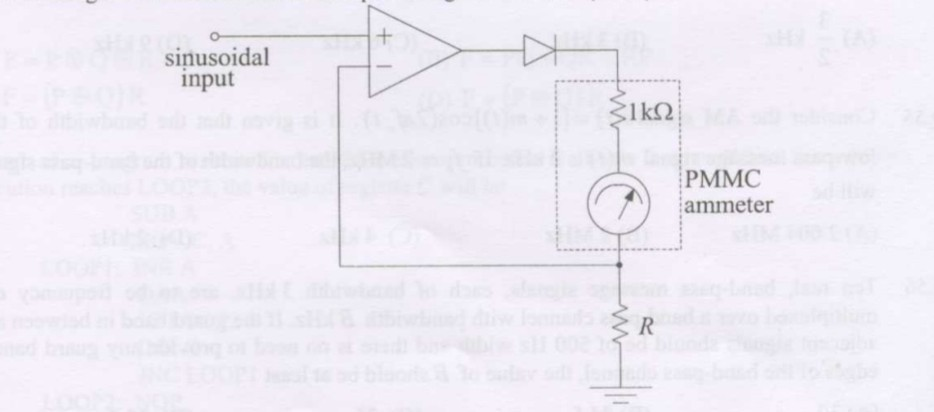
\includegraphics[width=0.5\columnwidth]{figs/i24.jpg}
    \caption{}
    \label{fig:placeholder24}
\end{figure}
\begin{multicols}{4}
           \begin{enumerate} 
              \item 45 $\ohm$   
              \item 67.5 $\ohm$
              \item 100 $\ohm$
              \item 144.4 $\ohm$
            \end{enumerate}
            \end{multicols}

\item  The x and y sensitivities of an analog oscilloscope are set as 2 ms/cm and 1V/cm respectively. The
trigger is set at $0 V$ with negative slope. An input of 2 $\cos{\brak{100{\pi}t + 30\degree}}$ V is fed to the y input of
the oscilloscope. The waveform seen on the oscilloscope will be \hfill{(GATE-IN 2008)}
\begin{multicols}{2}
           \begin{enumerate} 
              \item  
              \begin{figure}[H]
    \centering
    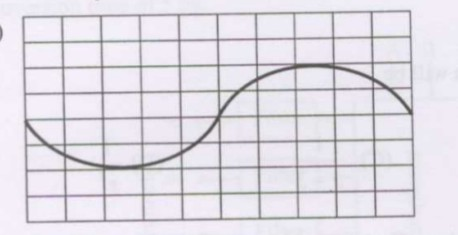
\includegraphics[width=0.5\columnwidth]{figs/i25.jpg}
    \caption{}
    \label{fig:placeholder25}
\end{figure}
              \item
              \begin{figure}[H]
    \centering
    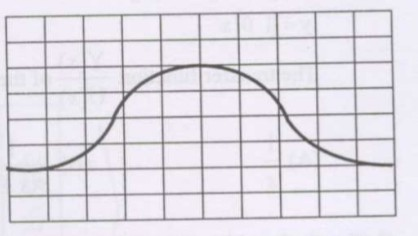
\includegraphics[width=0.5\columnwidth]{figs/i26.jpg}
    \caption{}
    \label{fig:placeholder26}
\end{figure}
              \item
              \begin{figure}[H]
    \centering
    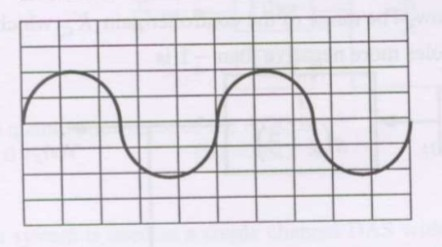
\includegraphics[width=0.5\columnwidth]{figs/i27.jpg}
    \caption{}
    \label{fig:placeholder27}
\end{figure}
              \item
              \begin{figure}[H]
    \centering
    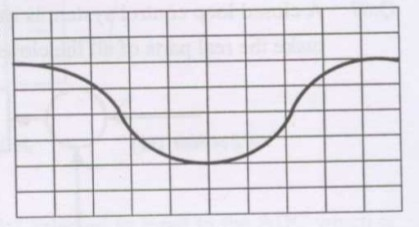
\includegraphics[width=0.5\columnwidth]{figs/i28.jpg}
    \caption{}
    \label{fig:placeholder28}
\end{figure}
            \end{enumerate}
\end{multicols}

\item The open loop transfer function of a unity feedback system is $G\brak{s}$ =$\frac{K\brak{s+2}}{\brak{s+1+j1}\brak{s+1-j1}}$. The root locus plot of the system has \hfill{(GATE-IN 2008)}
           \begin{enumerate} 
              \item two breakaway points located at s = -0.59 and s = -3.41 
              \item one breakaway point located at s = -0.59
              \item one breakaway point located at s =-3.41
              \item one breakaway point located at s =-1.41
            \end{enumerate}

\item If a first order system and its time response to a unit step input are as shown below in \figref{fig:placeholder29}, the gain K is \hfill{(GATE-IN 2008)}
\begin{figure}[H]
    \centering
    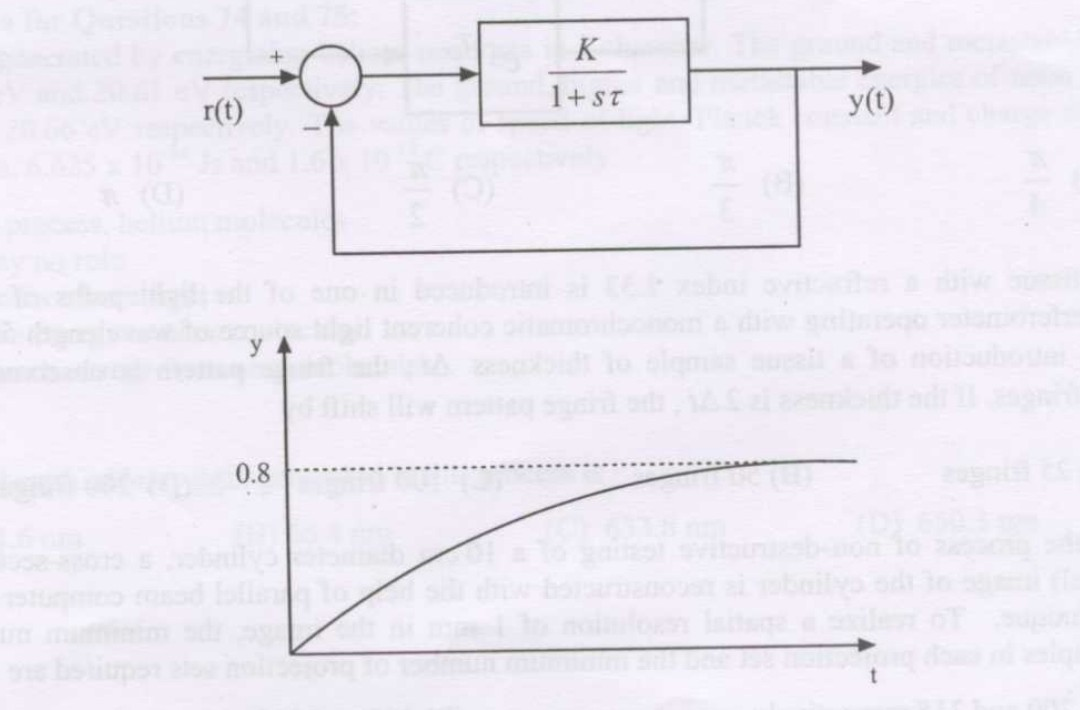
\includegraphics[width=0.5\columnwidth]{figs/i29.jpg}
    \caption{}
    \label{fig:placeholder29}
\end{figure}
\begin{multicols}{4}
           \begin{enumerate} 
              \item 0.25           
              \item 0.8
              \item 1
              \item 4
            \end{enumerate}
\end{multicols}

\item The state space representation of a system is given by \


\begin{align}
\dot{x} &= 
\myvec{
0 & 1 \\
0 & -3
} x
+ 
\myvec{
1 \\
0
} u
\\
y &= 
\myvec{
1 & 0
} x
\end{align}


The transfer function$\frac{Y\brak{s}}{U\brak{s}}$ of the system will be \hfill{(GATE-IN 2008)}
\begin{multicols}{4}
           \begin{enumerate} 
              \item $\frac{1}{s}$           
              \item $\frac{1}{s\brak{s+3}}$
              \item $\frac{1}{s+3}$
              \item $\frac{1}{s^2}$
            \end{enumerate}
            \end{multicols}

            
\item  A closed loop control system is shown below. \figref{fig:placeholder30} The range of the controller gain $K_{C}$  which will
make the real parts of all the closed loop poles more negative than -1 is \hfill{(GATE-IN 2008)}
\begin{figure}[H]
    \centering
    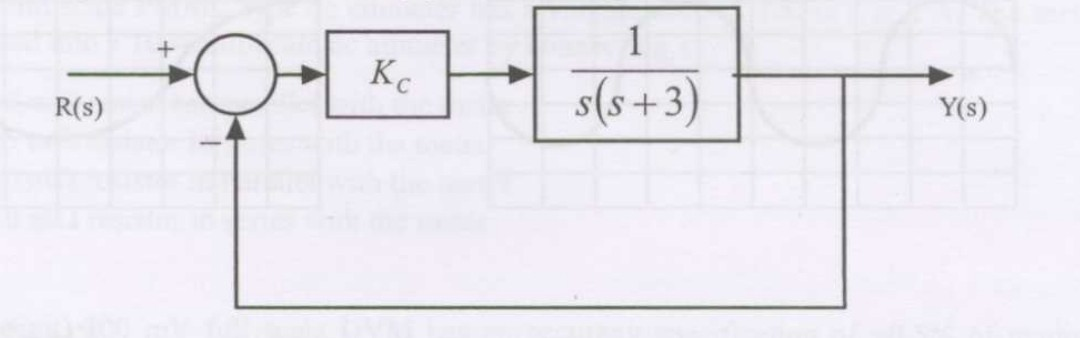
\includegraphics[width=0.5\columnwidth]{figs/i30.jpg}
    \caption{}
    \label{fig:placeholder30}
\end{figure}
\begin{multicols}{4}
           \begin{enumerate} 
              \item $K_C$ $>$ -4         
              \item $K_C$ $>$ 0
              \item $K_C$ $>$ 2
              \item $K_C$ $<$ 2
            \end{enumerate}
            \end{multicols}


\item For the closed loop system shown below \figref{fig:placeholder31} to be stable, the value of time delay $T_D$  $\brak{in seconds}$
should be less than \hfill{(GATE-IN 2008)}
\begin{figure}[H]
    \centering
    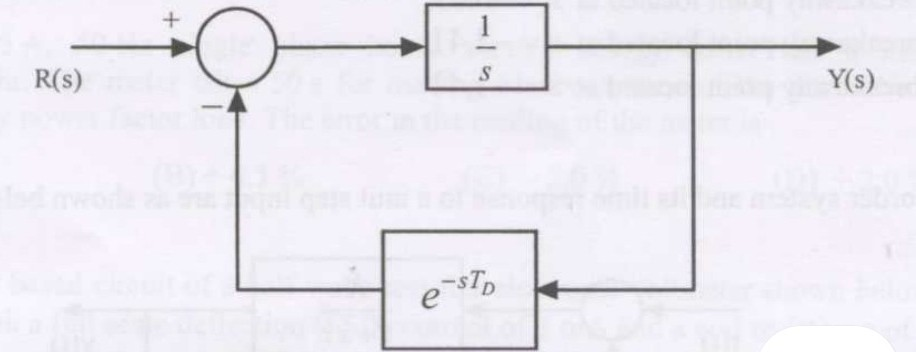
\includegraphics[width=0.5\columnwidth]{figs/i31.jpg}
    \caption{}
    \label{fig:placeholder31}
\end{figure}
\begin{multicols}{4}
           \begin{enumerate} 
              \item $\frac{\pi}{4}$           
              \item $\frac{\pi}{3}$           
              \item $\frac{\pi}{2}$           
              \item ${\pi}$           
            \end{enumerate} 
            \end{multicols}

\item A tissue with a refractive index 1.33 is introduced in one of the light paths of a Michelson
interferometer operating with a monochromatic coherent light source of wavelength 589 nm. After
the introduction of a tissue sample of thickness $\Delta$$t$, the fringe pattern is observed to shift by
50 fringes. If the thickness is 2 $\Delta$$t$ , the fringe pattern will shift by \hfill{(GATE-IN 2008)}
\begin{multicols}{4}
           \begin{enumerate} 
              \item 25 fringes        
              \item 50 fringes
              \item 100 fringes
              \item 200 fringes
            \end{enumerate}
            \end{multicols}

\item In the process of non-destructive testing of a 10 cm diameter cylinder, a cross-sectional \brak{transaxial} image of the cylinder is reconstructed with the help of parallel beam computer tomography
technique. To realize a spatial resolution of 1 mm in the image, the minimum number of ray
samples in each projection set and the minimum number of projection sets required are \hfill{(GATE-IN 2008)}
\begin{multicols}{2}
           \begin{enumerate} 
              \item  200 and 315 respectively          
              \item  100 and 315 respectively
              \item  200 and 629 respectively
              \item  100 and 629 respectively
            \end{enumerate}
            \end{multicols}


\section*{Common Data Questions}
\textbf{Common Data for Questions 71,72 and 73}
A data acquisition system \brak{DAS} shown below \figref{fig:placeholder32} employs a successive 
approximation type 12-bit ADC having a conversion time of $5$ $\mu$s.

\begin{figure}[H]
    \centering
    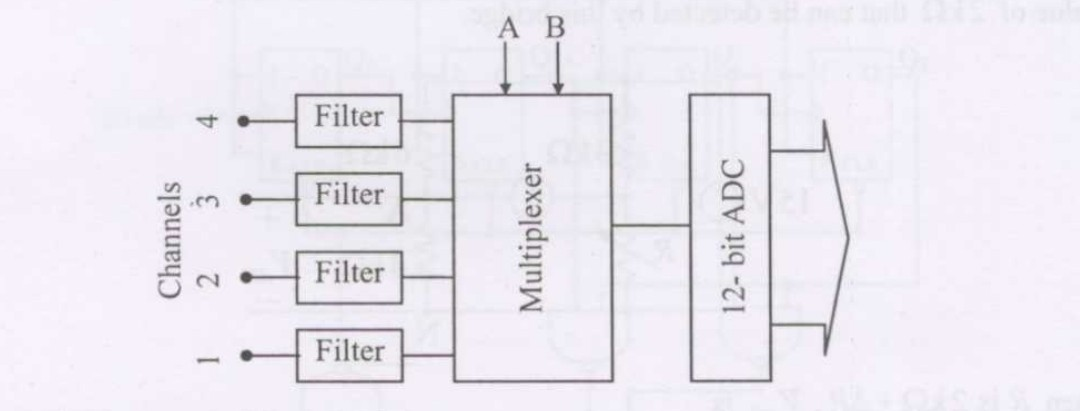
\includegraphics[width=0.5\columnwidth]{figs/i32.jpg}
    \caption{}
    \label{fig:placeholder32}
\end{figure}


            

\item The quantization error of the ADC is \hfill{(GATE-IN 2008)}
\begin{multicols}{4}
           \begin{enumerate} 
              \item 0           
              \item $\underset{-}{+}$ 0.012 \%
              \item $\underset{-}{+}$ 0.024 \%
              \item $\underset{-}{+}$ 0.048 \%
            \end{enumerate}
            \end{multicols}

\item  The system is used as a single channel DAS with channel 1 selected as input to the ADC which is
set in the continuous conversion mode. For avoiding aliasing error, the cutoff frequency $f_c$ of the
filter in channel 1 should be \hfill{(GATE-IN 2008)}
\begin{multicols}{2}
           \begin{enumerate} 
              \item $f_c$ $<$ 100 kHz         
              \item $f_c$ = 100kHz
              \item 100 kHz $<$ $f_c$ $<$ 200 kHz
              \item $f_c$ = 200 kHz
            \end{enumerate}
            \end{multicols}

\item If the multiplexer is controlled such that the channels are sequenced every 5 us as 1, 2, 1, 3, 1, 4, 1,
2, 1, 3, 1, 4, 1, ....., the input connected to channel 1 will be sampled at the rate of \hfill{(GATE-IN 2008)}
\begin{multicols}{4}
           \begin{enumerate} 
              \item 25k samples/s           
              \item 50k samples/s
              \item 100k samples/s
              \item 200k samples/s
            \end{enumerate}
            \end{multicols}

\textbf{Common Data for Questions 74 and 75}

Laser light is generated by energizing helium-neon gas in a chamber. The ground and metastable states of
helium are 0 eV and 20.61 eV respectively. The ground, higher and metastable energies of neon are 0 eV,
18.70 eV and 20.66 eV respectively. The values of speed of light, Planck constant and charge of electron
are 3 x $10^{8}$  m/s, 6.625 x $10^{-34}$ 4 Js and 1.6 x $10^{19}$ C respectively.


 \item In this process, helium molecules \hfill{(GATE-IN 2008)}
 \begin{multicols}{2}
           \begin{enumerate} 
              \item  play no role        
              \item  produce laser light
              \item  give energy to neon molecules
              \item  absorb energy from neon molecules
            \end{enumerate}
\end{multicols}


\item  Wavelength of laser light generated in this process is \hfill{(GATE-IN 2008)}
\begin{multicols}{4}
           \begin{enumerate} 
              \item 61.6 nm       
              \item 66.4 nm
              \item 633.8 nm
              \item 650.3 nm
            \end{enumerate}
            \end{multicols}

\section*{Linked Answer Questions: Q.76 to Q.85 carry two marks each }
\textbf{Statement for Linked Answer Questions 76 and 77:}

In the Wheatstone bridge shown below \figref{fig:placeholder33} the galvanometer G has a current sensitivity of 1 $\mu$A/mm, a
resistance of 2.5 k$\ohm$and a scale resolution of 1 mm. Let $\Delta$$R$ be the minimum increase in R from its
nominal value of 2k$\ohm$ that can be detected by this bridge.

\begin{figure}[H]
    \centering
    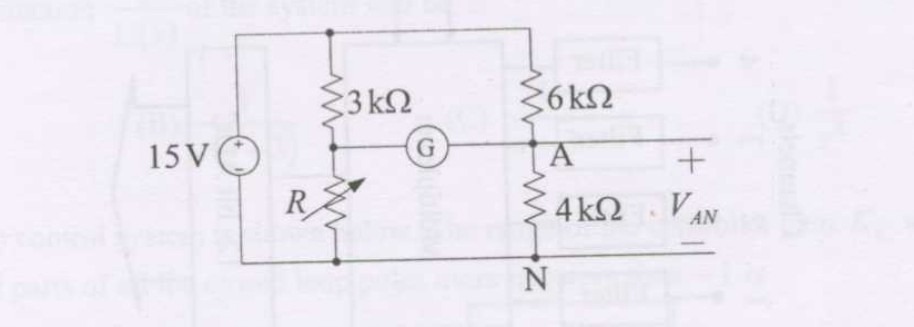
\includegraphics[width=0.5\columnwidth]{figs/i33.jpg}
    \caption{}
    \label{fig:placeholder33}
\end{figure}

\item When R is 2k$\ohm$ + $\Delta$$R$ , $V_{AN}$ is \hfill{(GATE-IN 2008)}
\begin{multicols}{4}
           \begin{enumerate} 
              \item 6 V
              \item 6.0024 V
              \item 6.0038 V
              \item 6.005 V
            \end{enumerate}
            \end{multicols}




\item The value of $\Delta$$R$ is approximately \hfill{(GATE-IN 2008)}
\begin{multicols}{4}
           \begin{enumerate} 
              \item  2.8 $\ohm$       
              \item  3.4 $\ohm$
              \item  5.2 $\ohm$
              \item  12 $\ohm$
            \end{enumerate}
            \end{multicols}

\textbf{Statement for Linked Answer Questions 78 and 79:}

In the circuit shown below \figref{fig:placeholder34} the steady-state is reached with the switch K open. Subsequently the switch is
closed at time t = 0.

\begin{figure}[H]
    \centering
    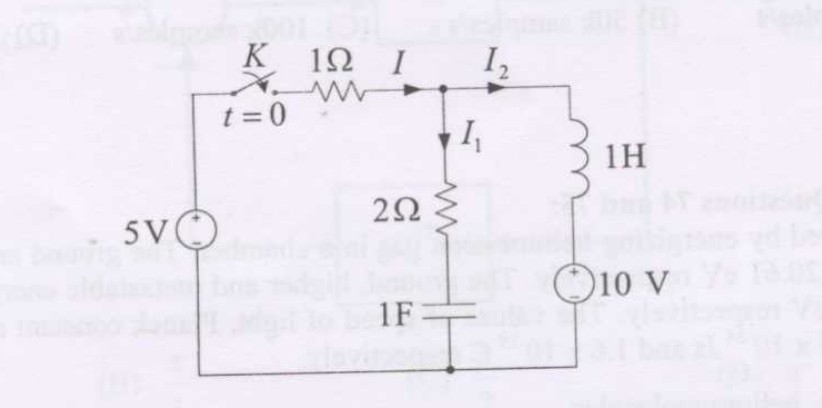
\includegraphics[width=0.3\columnwidth]{figs/i34.jpg}
    \caption{}
    \label{fig:placeholder34}
\end{figure}

\item  At time t = $0^{+}$, current I is \hfill{(GATE-IN 2008)}
\begin{multicols}{4}
           \begin{enumerate} 
              \item  -$\frac{5}{3}$ A    
              \item  0 A
              \item  $\frac{5}{3}$ A
              \item  $\infty$ A
            \end{enumerate}
            \end{multicols}


\item At time t = $0^{+}$, $\frac{dI_2}{dt}$ \hfill{(GATE-IN 2008)}
\begin{multicols}{4}
           \begin{enumerate} 
              \item  -5 A/s       
              \item  -$\frac{10}{3}$ A/s 
              \item  0 A/s
              \item  5A/s
            \end{enumerate}
            \end{multicols}

\textbf{Statement for Linked Answer Questions 80 and 81 :}

Consider the counter circuit shown below.\figref{fig:placeholder35}
\begin{figure}[H]
    \centering
    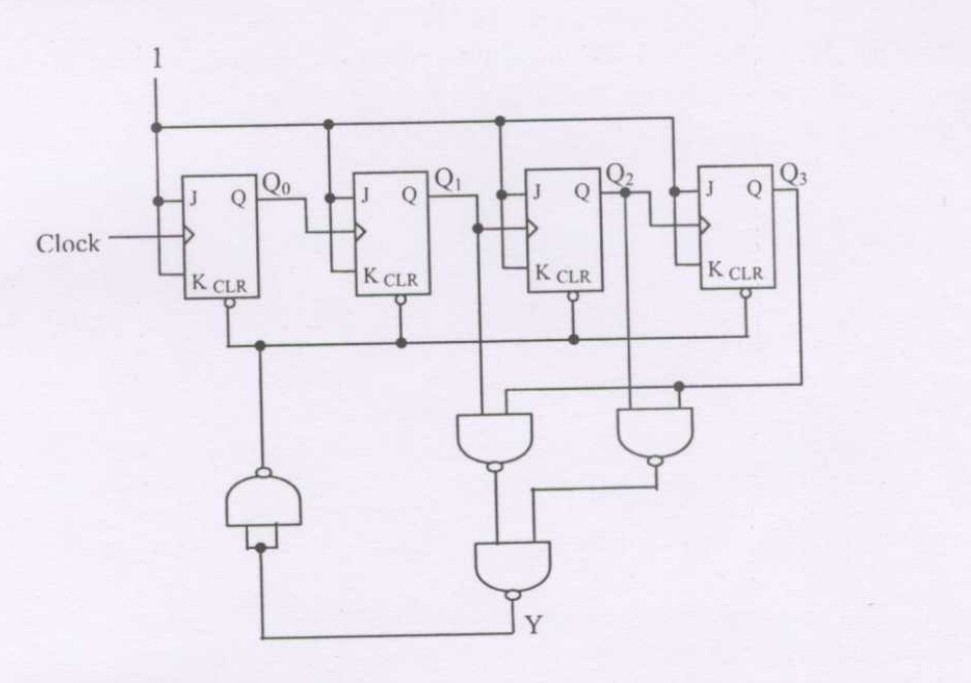
\includegraphics[width=0.5\columnwidth]{figs/i35.jpg}
    \caption{}
    \label{fig:placeholder35}
\end{figure}

\item  In the above figure, Y can be expressed as \hfill{(GATE-IN 2008)}
\begin{multicols}{4}
           \begin{enumerate} 
              \item $Q_3 \brak{Q_2 + Q_1}$        
              \item  $Q_3$ + $Q_2$$Q_1$
              \item $\overline{Q_3\brak{Q_2 + Q_1}}$
              \item $\overline{Q_3 + Q_2  Q_1}$ 
            \end{enumerate}
            \end{multicols}


\item The above circuit is a \hfill{(GATE-IN 2008)}
\begin{multicols}{4}
           \begin{enumerate} 
              \item  Mod-8 Counter           
              \item  Mod-9 Counter
              \item  Mod-10 Counter
              \item  Mod-11 Counter
            \end{enumerate}
            \end{multicols}

\textbf{Statement for Linked Answer Questions 82 and 83 :}

Consider a unity feedback system with open loop transfer function $G\brak{s}$ = $\frac{1+ 6s}{s^2\brak{1+s}\brak{1+2s}}$



\item The phase crossover frequency of the system in radians per second is \hfill{(GATE-IN 2008)}
\begin{multicols}{4}
           \begin{enumerate} 
              \item 0.125            
              \item 0.25
              \item 0.5
              \item 1
            \end{enumerate}
            \end{multicols}

\item The gain margin of the system is \hfill{(GATE-IN 2008)}
\begin{multicols}{4}
           \begin{enumerate} 
              \item  0.125          
              \item  0.25
              \item  0.5
              \item  1
            \end{enumerate}
            \end{multicols}

\textbf{Statement for Linked Answer Questions 84 and 85 :}

A unity feedback system has open loop transfer function $G\brak{s}$ = $\frac{100}{s\brak{s+p}}$. The time at which the
response to a unit step input reaches its peak is $\frac{\pi}{8}$ seconds.




\item The damping coefficient for the closed loop system is \hfill{(GATE-IN 2008)}
\begin{multicols}{4}
           \begin{enumerate} 
              \item  0.4      
              \item  0.6
              \item  0.8
              \item  1
            \end{enumerate}
            \end{multicols}


\item The value of p is \hfill{(GATE-IN 2008)}
\begin{multicols}{4}
           \begin{enumerate} 
              \item 6           
              \item 12
              \item 14
              \item 16
            \end{enumerate}
\end{multicols}


\end{enumerate}

\end{document}
